\chapter{Experimenteller Aufbau}
\label{chap:experiment}

\noindent Im folgenden wird nun der experimentelle Aufbau zur Messung der Transmissionsspektren betrachtet und die verwendeten Bauteile erklärt. Dazu werden sämtliche Informationen der Versuchsanleitung \cite{H2} entnommen und zur Vollständigkeit gebündelt dargestellt.\\


\noindent Da die verwendete Laserdiode aufgrund ihrer Bauweise und Geometrie einen stark elliptischen Strahl emittiert, muss dieser unter Verwendung des \textbf{anamorphotischen Prismenpaares}, bestehend aus zwei jeweils $30^\circ$ Prismen, in eine runde Form gebracht werden, um die Einkopplung eines Teilstrahls gemäß Abbildung \ref{fig:Versuchsaufbau-Abs} in den konfokalen \textbf{Referenzresonator} mit $R_{c}=\SI{10}{\centi \meter}$ zu gewährleisten.\\
\noindent Die Implimentierung des \textbf{optischen Isolators} in den Versuchsaufbau ist notwendig, um potentielle Rückreflexe zu filtern und so einen stabilen Laserbetrieb sicher zu stellen. Das Funktionsprinzp basiert auf einem optisch aktiven Medium -- meist dotiertem Glas -- in einem starken Magnetfeld, wodurch mittels dem Faraday-Effekt linear polarisiertes Licht um $45^\circ$ rotiert wird. Zusätzlich befinden sich vor und nach dem Glas Polarisatoren, die um $45^\circ$ zueinander verdreht stehen. Der erste Polarisator ist parallel zur Durchlassrichtung des eintretenden Laserstrahls positioniert, um eine Propagation durch den Isolator zu erlauben. Da die Rückreflexe durch den Faraday-Effekt senkrecht zur Durchlassrichtung auf den ersten Polarisator treffen, werden diese dort absorbiert.\\
\noindent In Abbildung \ref{fig:Versuchsaufbau-Abs} ist eine schematische Darstellung des Versuchsaufbaus für die Absorptionsspektroskipie zu sehen. Nachdem der Strahl für ein Referenzsignal geteilt wurde, passiert der transmittierte Teil eine \textbf{$\frac{\lambda}{2}$}--Platte und wird in seiner Polarisationsrichtung um $\pi$ gedreht, um anschließend unter Verwendung eines \textbf{polarisierenden Strahlteilers} in seine s--polarisierte und p--polarisierte Komponenten aufgeteilt zu werden. Der p--polarisierte Strahl trifft auf die Probe in der \textbf{Rubidium Zelle}, während der s--polarisierte Teil reflektiert wird. \\
\noindent Zur Qualitätsoptimierung der Messung wird der Strahl mittels einer plankonvexen \textbf{Linse} auf die \textbf{Photodiode} fokussiert um die maximale Intensität detektieren zu können. Indem ein \textbf{Bandpass}, der auf die Laserwellenlänge von $(780 \pm 5)$nm abgestimmt ist, vor die Photodiode geschaltet wird, reduziert sich der störende Einfluss des aus der Umgebung kommenden Lichtes auf ein Minimum und das Signal kann näherungsweise als störungsfrei angenommen werden.

\begin{comment}
\begin{figure}[!h]
    \centering
    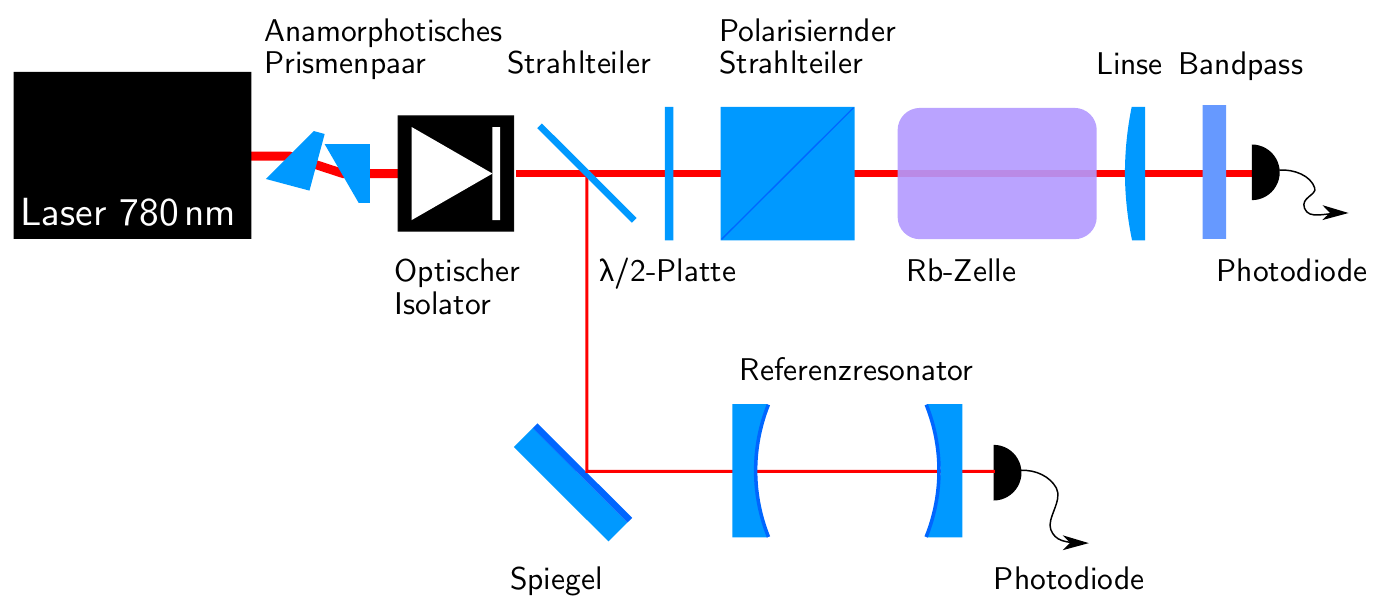
\includegraphics[scale = 0.5]{figures/images/absorp-aufbau.png}
    \caption{Aufbau Absorptionsspektroskopie [Quelle: \cite{H2}, S. 32]}
    \label{fig:Versuchsaufbau-Abs}
\end{figure}

\begin{figure}[!h]
    \centering
    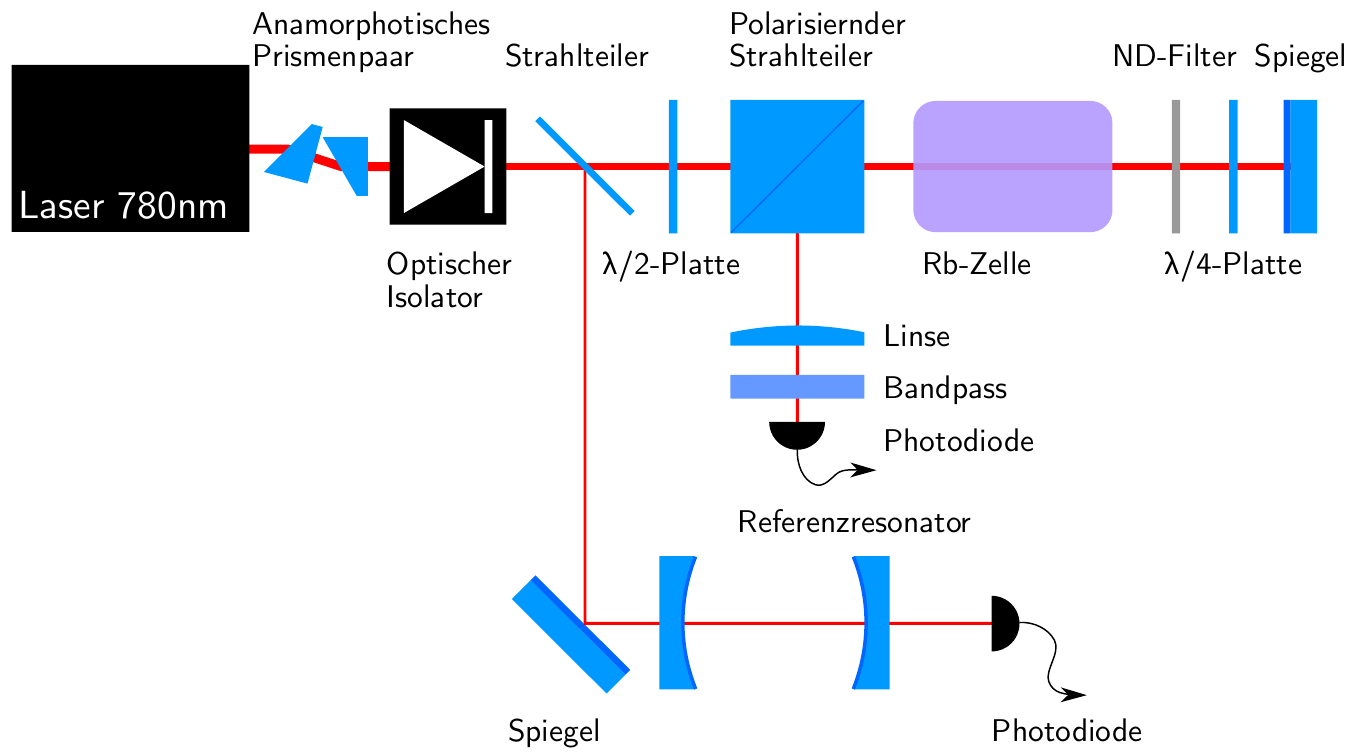
\includegraphics[scale = 0.5]{figures/images/saettig-aufbau.png}
    \caption{Aufbau Sättigungsspektroskopie [Quelle: \cite{H2}, S. 36]}
    \label{fig:Versuchsaufbau-Saet}
\end{figure}
\end{comment}

%\begin{comment}
\begin{figure}[!h]
    \begin{minipage}{8cm}
        \centering
        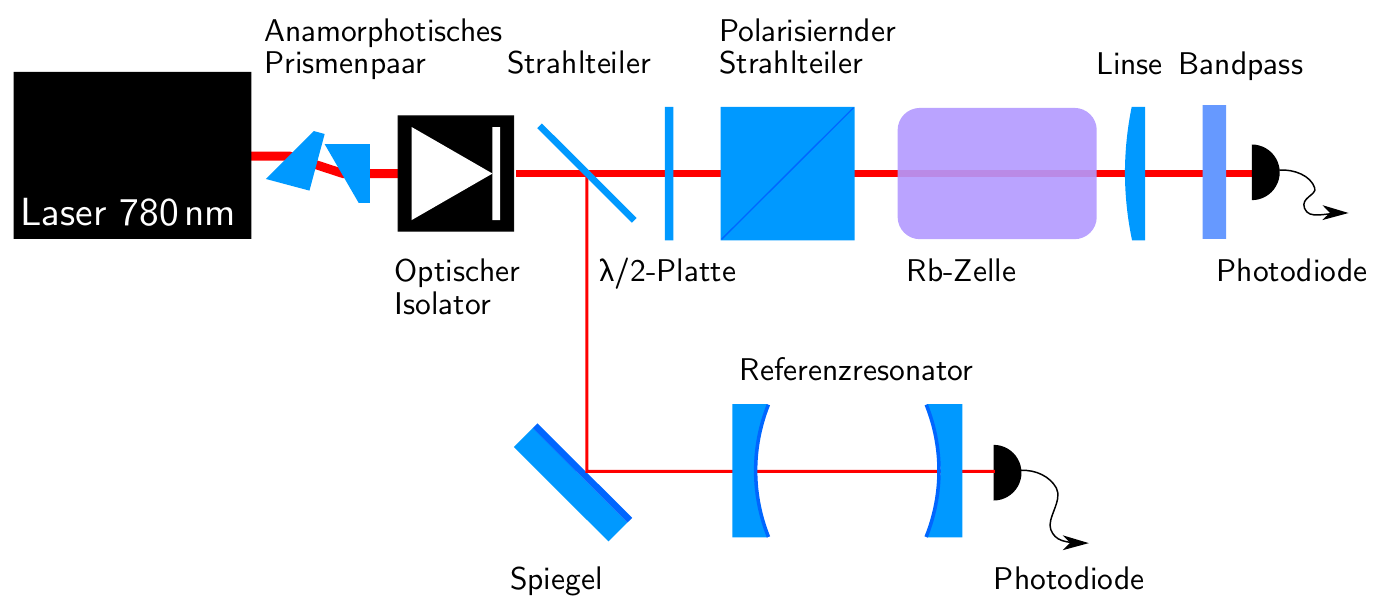
\includegraphics[scale = 0.30]{figures/images/absorp-aufbau.png}
        \caption{Aufbau Absorptionsspektroskopie [Quelle: \cite{H2}, S. 32]}
        \label{fig:Versuchsaufbau-Abs}
    \end{minipage}
    \hfill
    \begin{minipage}{8cm}
        \centering
        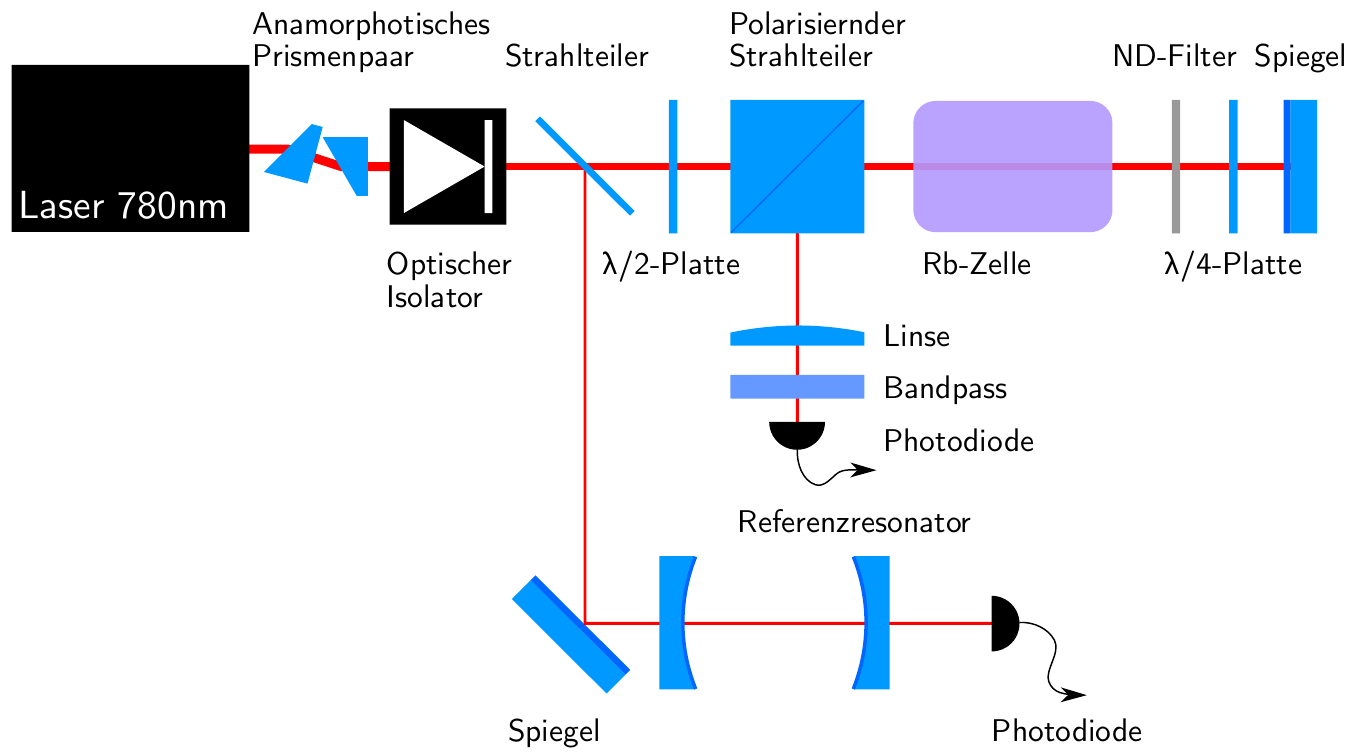
\includegraphics[scale = 0.25]{figures/images/saettig-aufbau.png}
        \caption{Aufbau Sättigungsspektroskopie [Quelle: \cite{H2}, S. 36]}
        \label{fig:Versuchsaufbau-Saet}
    \end{minipage}
\end{figure}
%\end{comment}

\noindent Der Versuchsaufbau für die Sättigungsspektroskopie aus Abbildung \ref{fig:Versuchsaufbau-Saet} unterscheidet sich im Wesentlichen darin, dass das Kollektiv bestehend aus Linse, Bandpass und Photodiode nun auf den reflektierten Strahl aus dem polarisierenden Strahlteiler fokussiert wird. An die Ursprüngliche Position der Photodiode kommt ein Kombination aus \textbf{ND-Filter}, \textbf{$\frac{\lambda}{4}$}--Platte und \textbf{Spiegel}, um den aus Kapitel 2.2.3 erläuterten Teststrahl zu erzeugen. Dabei reduziert der ND-Filter die Intensität des durchlaufenden Strahls um $T=10^{-D(\lambda)}$. In diesem Fall bezeichnet $D(\lambda)=\log(1-\E^{-\alpha(\lambda) \cdot \ell})$ die optische Dichte, $\alpha(\lambda)$ den Absorptionskoeffizienten nach dem \textit{Lambert-Beerschen Gesetz} und $\ell$ die Strecke auf der es zur Absorption kommt. \\
\noindent Aufgrund der $\frac{\lambda}{4}$--Platte, die bei jedem Durchgang die Phase um $\frac{\pi}{2}$ verzögert und dem Phasensprung um $\pi$, der beim Übergang vom optisch dünneren ins optisch dichtere Medium zustande kommt, befindet sich der Teststrahl beim Durchlaufen der Probe in Phase mit dem Pumpstrahl. Im Experiment wird dafür das Plättchen in der $x$-$y$ Ebene (unter der Annahme die optische Achse liege parallel zur $z$-Achse) so lange rotiert, bis die Peaks des Intensitätsverlaufs auf dem Oszilloskop maximal werden.

\noindent Auf die für den Laserbetrieb notwendige Elektronik wie Temperatur- und Stromcontroller, Funktionsgenerator und Oszilloskop oder Spannungsaddierer wird an dieser Stelle nicht explizit eingegangen. Diesbezüglich sind sämtliche Informationen der Versuchsanleitung \cite{H2} zu entnehmen. \\
\noindent Während des Versuchs wurden alle Parameter laufend überwacht und können als konstant angenommen werden. Durch die vom Funktionsgenerator ausgegebene Dreiecksfunktion konnte die Laserfrequenz moduliert werden.\\

\noindent Nachdem sowohl die theoretischen Grundlagen, als auch der experimentelle Aufbau ausführlich diskutiert worden sind, beschäftigt sich das nächste Kapitel dieser Arbeit mit der Auswertung unserer Messwerte.

\cleardoublepage{}